%
% This is a borrowed LaTeX template file for lecture notes for CS267,
% Applications of Parallel Computing, UCBerkeley EECS Department.
% Now being used for CMU's 10725 Fall 2012 Optimization course
% taught by Geoff Gordon and Ryan Tibshirani.  When preparing 
% LaTeX notes for this class, please use this template.
%
% To familiarize yourself with this template, the body contains
% some examples of its use.  Look them over.  Then you can
% run LaTeX on this file.  After you have LaTeXed this file then
% you can look over the result either by printing it out with
% dvips or using xdvi. "pdflatex template.tex" should also work.
%

\documentclass[twoside]{article}
\setlength{\oddsidemargin}{0.25 in}
\setlength{\evensidemargin}{-0.25 in}
\setlength{\topmargin}{-0.6 in}
\setlength{\textwidth}{6.5 in}
\setlength{\textheight}{8.5 in}
\setlength{\headsep}{0.75 in}
\setlength{\parindent}{0 in}
\setlength{\parskip}{0.1 in}

%
% ADD PACKAGES here:
%

\usepackage{amsmath,amsfonts,graphicx}

%
% The following commands set up the lecnum (lecture number)
% counter and make various numbering schemes work relative
% to the lecture number.
%
\newcounter{lecnum}
\renewcommand{\thepage}{\thelecnum-\arabic{page}}
\renewcommand{\thesection}{\thelecnum.\arabic{section}}
\renewcommand{\theequation}{\thelecnum.\arabic{equation}}
\renewcommand{\thefigure}{\thelecnum.\arabic{figure}}
\renewcommand{\thetable}{\thelecnum.\arabic{table}}

%
% The following macro is used to generate the header.
%
\newcommand{\lecture}[4]{
   \pagestyle{myheadings}
   \thispagestyle{plain}
   \newpage
   \setcounter{lecnum}{#1}
   \setcounter{page}{1}
   \noindent
   \begin{center}
   \framebox{
      \vbox{\vspace{2mm}
    \hbox to 6.28in { {\bf EE402 - Discrete Time Systems
	\hfill Spring 2018} }
       \vspace{4mm}
       \hbox to 6.28in { {\Large \hfill Lecture #1 \hfill} }
       \vspace{2mm}
       \hbox to 6.28in { {\it Lecturer: #2 \hfill } }
      \vspace{2mm}}
   }
   \end{center}
   \markboth{Lecture #1}{Lecture #1}

   \vspace*{4mm}
}
%
% Convention for citations is authors' initials followed by the year.
% For example, to cite a paper by Leighton and Maggs you would type
% \cite{LM89}, and to cite a paper by Strassen you would type \cite{S69}.
% (To avoid bibliography problems, for now we redefine the \cite command.)
% Also commands that create a suitable format for the reference list.
\renewcommand{\cite}[1]{[#1]}
\def\beginrefs{\begin{list}%
        {[\arabic{equation}]}{\usecounter{equation}
         \setlength{\leftmargin}{2.0truecm}\setlength{\labelsep}{0.4truecm}%
         \setlength{\labelwidth}{1.6truecm}}}
\def\endrefs{\end{list}}
\def\bibentry#1{\item[\hbox{[#1]}]}

%Use this command for a figure; it puts a figure in wherever you want it.
%usage: \fig{NUMBER}{SPACE-IN-INCHES}{CAPTION}
\newcommand{\fig}[3]{
			\vspace{#2}
			\begin{center}
			Figure \thelecnum.#1:~#3
			\end{center}
	}
% Use these for theorems, lemmas, proofs, etc.
\newtheorem{theorem}{Theorem}[lecnum]
\newtheorem{lemma}[theorem]{Lemma}
\newtheorem{proposition}[theorem]{Proposition}
\newtheorem{claim}[theorem]{Claim}
\newtheorem{corollary}[theorem]{Corollary}
\newtheorem{definition}[theorem]{Definition}
\newenvironment{proof}{{\bf Proof:}}{\hfill\rule{2mm}{2mm}}

% **** IF YOU WANT TO DEFINE ADDITIONAL MACROS FOR YOURSELF, PUT THEM HERE:

\begin{document}

% Lecture Details
\lecture{7}{Asst. Prof. M. Mert Ankarali}

\par

\section*{Mapping Between s \& z Planes}

When the (uniform) impulse sampling is involved in the process, 
then we know that $s$ and $z$ variables are related with
%
\begin{align*}
  z = e^{Ts}
\end{align*}
%
which is a mapping from complex plane to complex plane, i.e. $M:
\mathbb{C} \mapsto \mathbb{C}$, where $M(s) = e^{Ts}$. We will analyze
different cases of this mapping and their relevance and importance. 

Morever, if $s_p$ is a pole of $G_p(s)$, then it is straightforward to
show that $z_p = e^{T s_p}$ is a pole of $G(z) = \mathcal{Z}\lbrace
G_p(s) \rbrace$ (as well as $G(z) = (1 - z^{-1}) \mathcal{Z}\lbrace
G(s)/s \rbrace$). 

Since poles of an LTI system (CT or DT) are the major features
that defines the stability and some other performance metrics,
analyzing this mapping is very critical for analyzing discrete 
time control systems.

\paragraph{Mapping of real line (left half and right half):} 

When $s$ is purely real (i.e. when the roots of the CT plant
are real) we have
 %
\begin{align*}
s &= \sigma \quad , \ \sigma \in \mathbb{R} \\
z &= e^{Ts} = e^{T \sigma} \quad , \ z \in \mathbb{R}^+
\end{align*}
%
It is also easy to see the difference between left half and right half
of the real line 
 %
\begin{align*}
\mathrm{If} \ \sigma \leq &= 0 \quad \rightarrow \quad z = e^{\sigma T}
  \in [0,1] \\
\mathrm{If} \ \sigma \geq &= 0 \quad \rightarrow \quad z = e^{\sigma T}
  \in [1,\infty)
\end{align*}
%
Mapping of both left and right real lines to z-plane is illustrated in
the Figure below. It can be seen that when $\sigma > 0$, $z > 1$, and 
similarly when $\sigma < 0$, $z < 1$. Technically on both planes
red curves belong to ``unstable'' behaviors, where as blue curves belong 
to ``stable'' behaviors.
%
    \begin{center}
\begin{minipage}[h]{0.75\linewidth}
    \begin{center}
      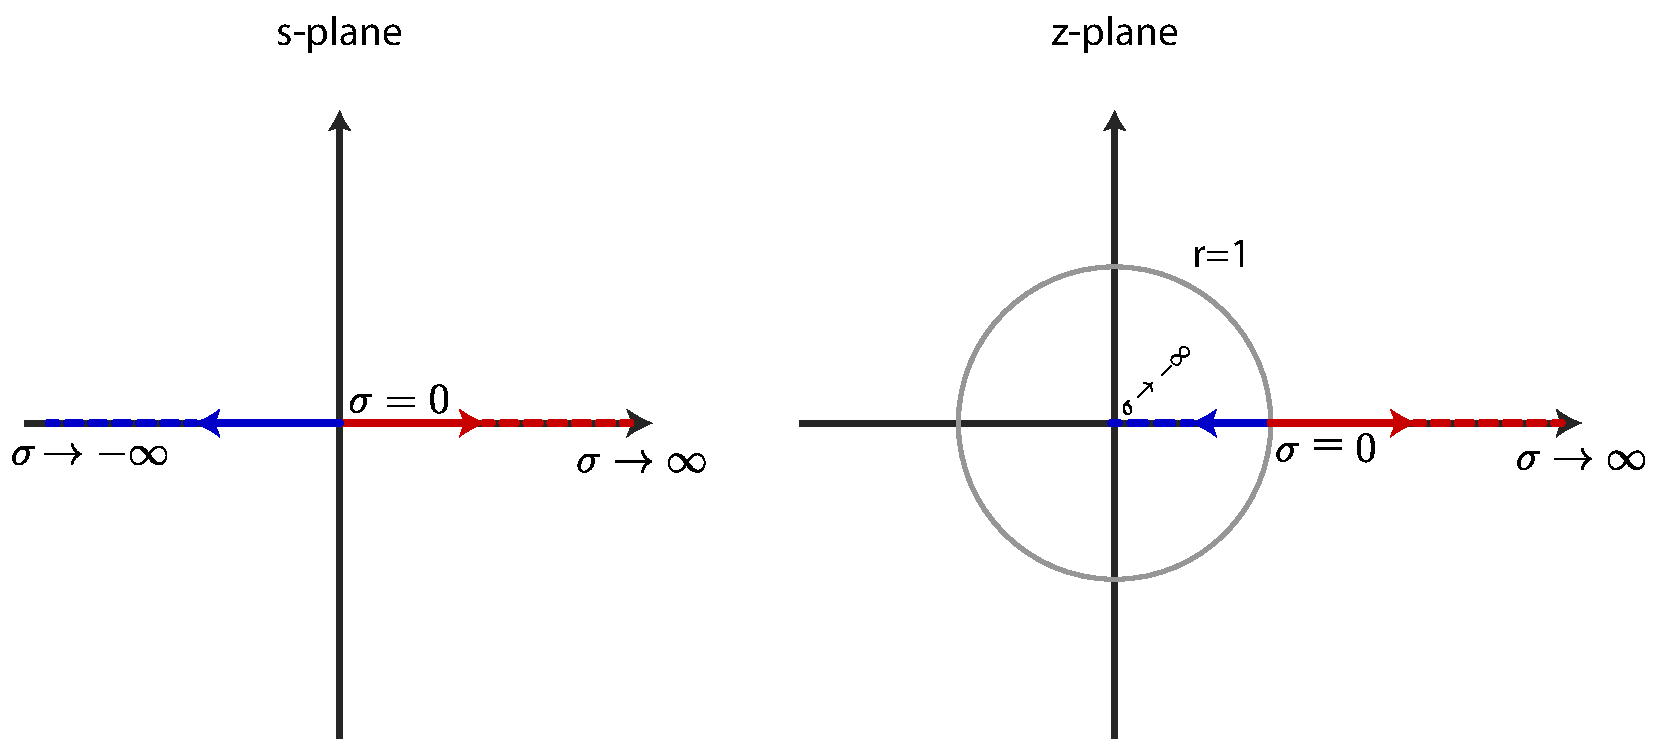
\includegraphics[width=\textwidth]{real}
    \end{center}
\end{minipage}
    \end{center}
%
\paragraph{Mapping of imaginary axis:} 
%
When $s$ is purely imaginary (i.e. when the roots of the CT plant
are critically stable) we have
 %
\begin{align*}
s &= j \omega \quad , \ \omega \in \mathbb{R} \\
z &= e^{Ts} = e^{T \omega j} \\
| z | &= 1 \\ 
\angle z &=  T \omega = T \omega + 2 \pi k  \quad , \ k \in \mathbb{Z}
\end{align*}
%
This means that mapping of the imaginary axis is not 1-1, since
multiple points on s plane can correspond to a single point on the 
z plane
%
\begin{align*}
e^{T \omega j} = e^{ \left( T \omega + 2 \pi k \right) j} \quad \rightarrow \quad
  M(\omega j) = M ( (\omega + 2\pi k / T) j ) =  M ( (\omega +
  \omega_s k) j ) \ , \ k \in \mathbb{Z}
\end{align*}
%
where $\omega_s = 2\pi / T$ is the sampling frequency. It can be seen
that imaginary axis on the s plane is mapped to the unit circle on the
z plane. However as $\omega \to \infty$ or $\omega \to -\infty$, 
the mapping circles the unit circle multiple (indeed infinite)
times. This mapping is illustrated in the Figure below. The light blue 
section on the s plane (which covers the points in the imaginary axis
between $[-\omega_s/2 , \omega_s/2]$) is called the primary
section/strip and fully mapped to the unit cicle. Dark blue sections
are called complementary sections/strips and they are also
individually fully mapped onto the unit circle. 
%
    \begin{center}
\begin{minipage}[h]{0.75\linewidth}
    \begin{center}
      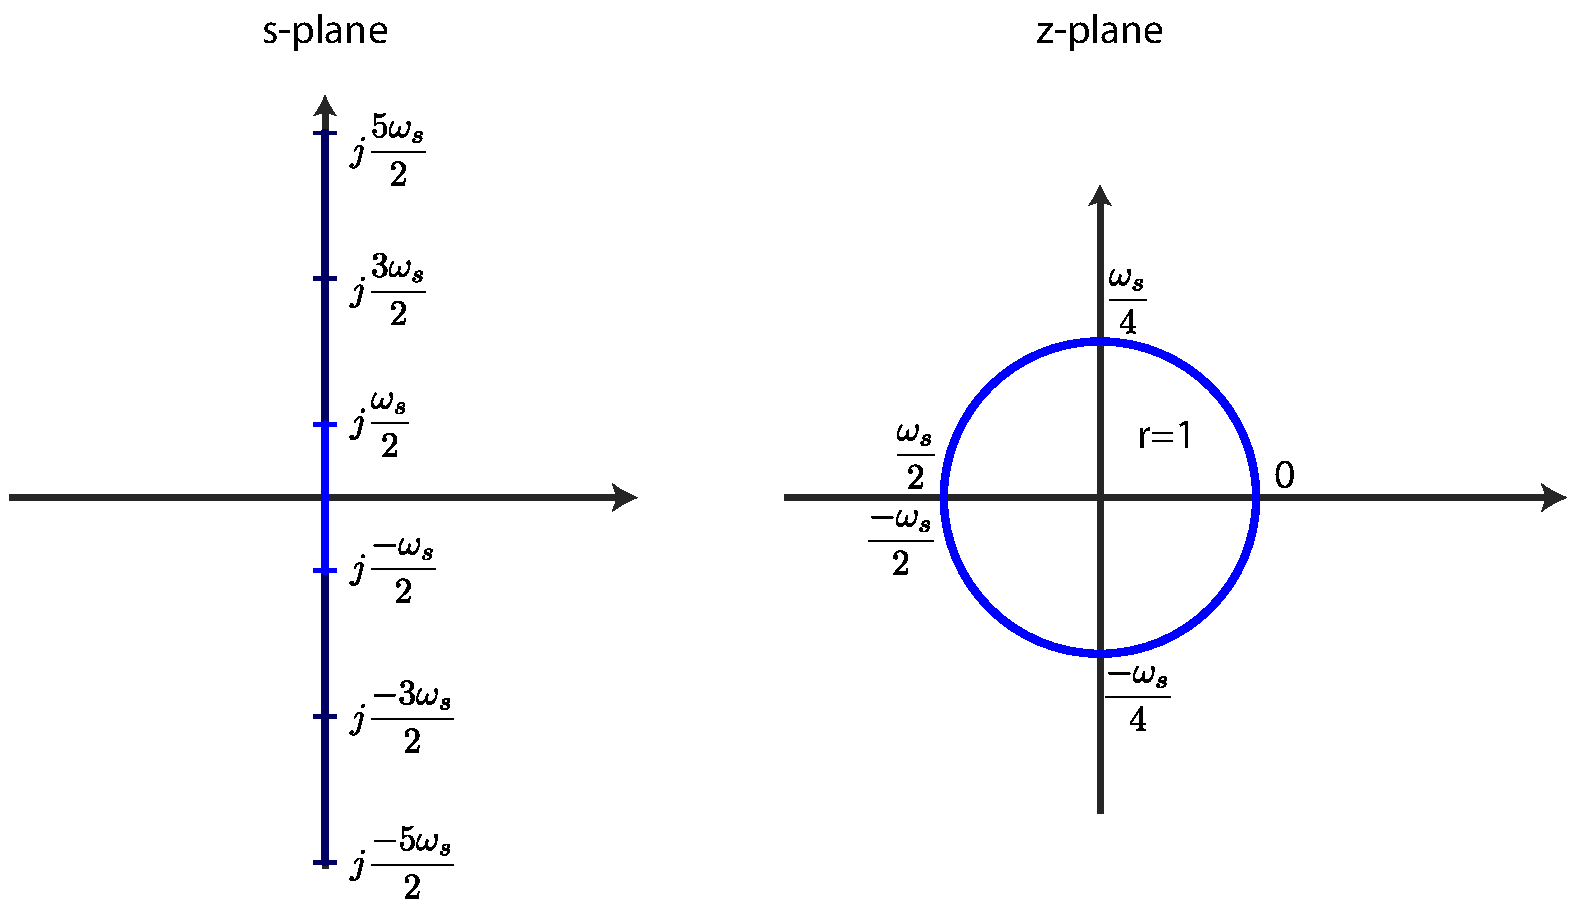
\includegraphics[width=\textwidth]{imag}
    \end{center}
\end{minipage}
    \end{center}
%
\paragraph{Mapping of open left-half plane:} 
%
Now let's generalize a little, and consider the mapping of the whole
open left-half plane.
%
\begin{align*}
s &= \sigma + j \omega \quad , \ \sigma < 0\\
z &= e^{Ts} = e^{T \sigma} e^{T \omega j} =  e^{T \sigma} e^{(T \omega
    + 2\pi k )j } \\
| z | &= e^{T \sigma} < 1 \\ 
\angle z &= T \omega + 2 \pi k  \quad , \ k \in \mathbb{Z}
\end{align*}
%
Obviously, this mapping is also not 1-1, and ``periodic'' in $\omega$, i.e.
\begin{align*}
  M(\sigma + \omega j ) = M (\sigma +  (\omega + 2\pi T) j ) =  M ( \sigma
  + (\omega + \omega_s) j )
\end{align*}
%
Mapping of OLH on s-plane to z-plane is illustrated in Figure below. 
%
    \begin{center}
\begin{minipage}[h]{0.85\linewidth}
    \begin{center}
      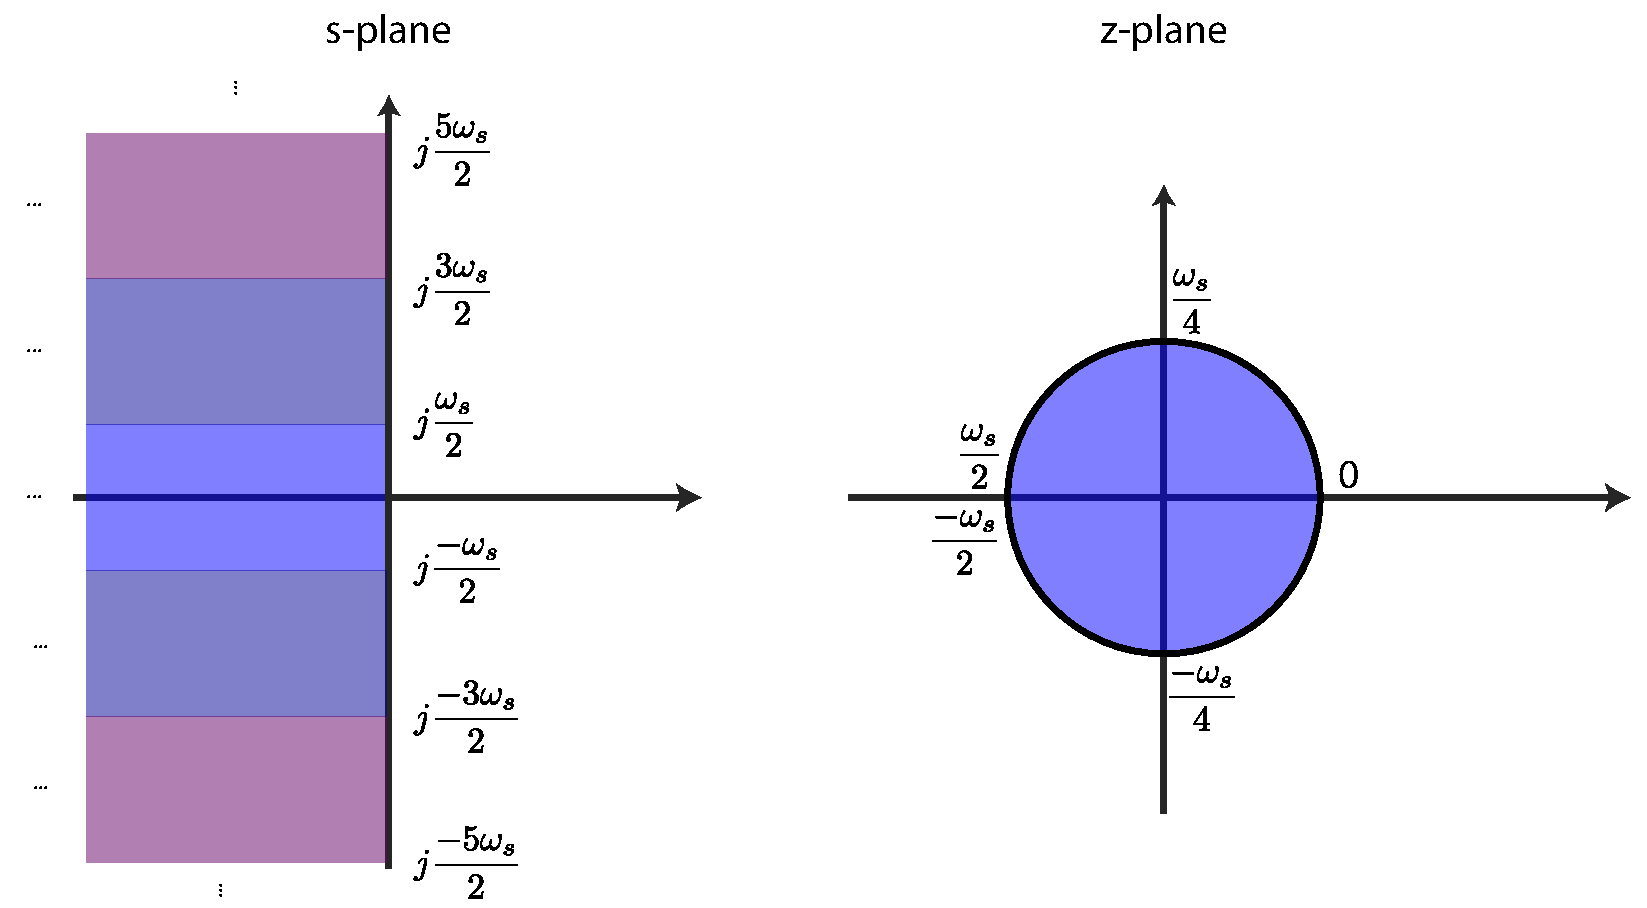
\includegraphics[width=\textwidth]{olh}
    \end{center}
\end{minipage}
    \end{center}
%
In the primary strip, if we trace the path that is defined by the
sequence of points 1-2-3-4-5-1 in the s plane as shown in the 
Figure below, than this path is mapped in to the z-plane as shown
in the Figure. The mapping forms a different path again associated
with mapped point sequence 1-2-3-4-5-1. 
%
    \begin{center}
\begin{minipage}[h]{0.95\linewidth}
    \begin{center}
      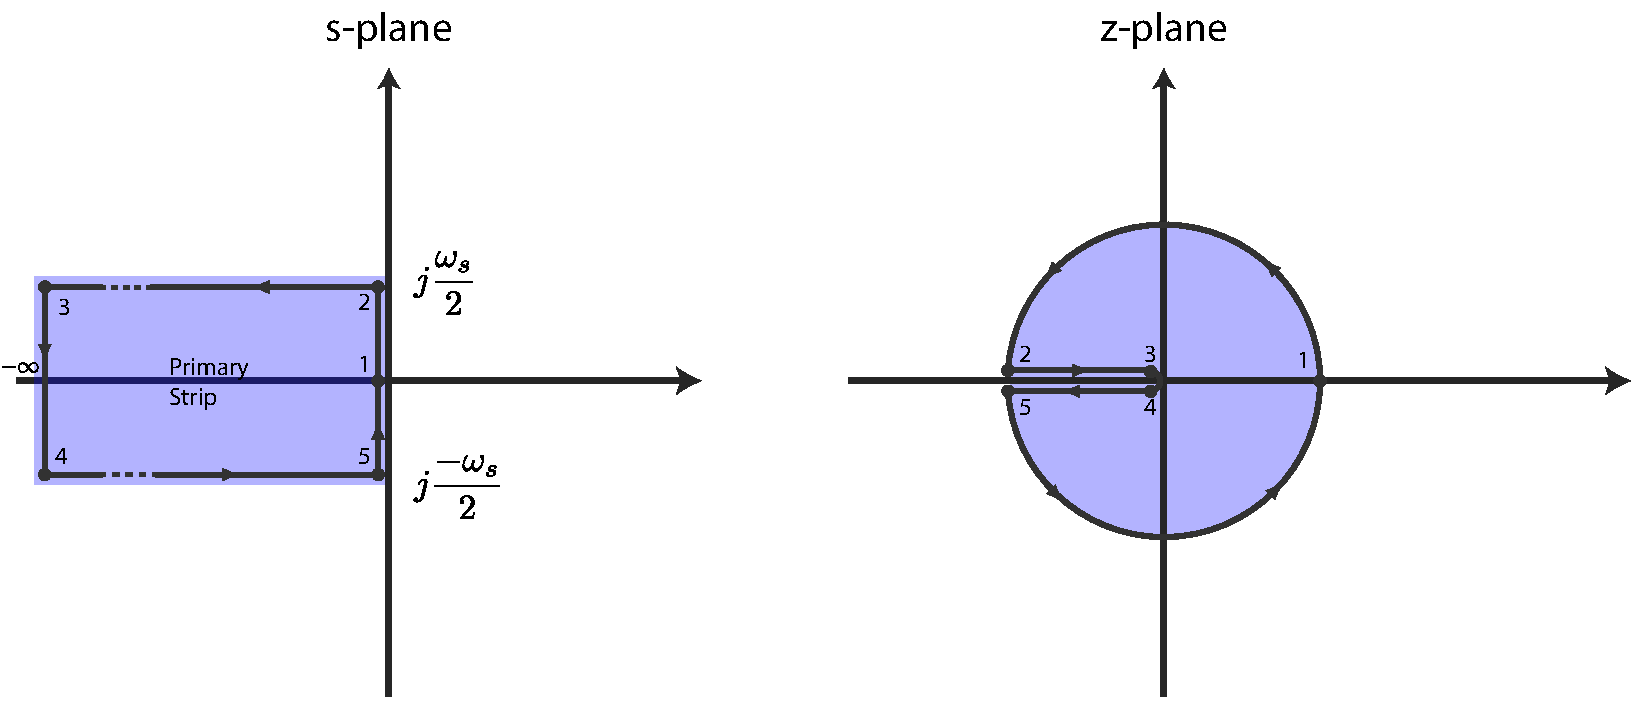
\includegraphics[width=\textwidth]{primary}
    \end{center}
\end{minipage}
    \end{center}
%
\paragraph{Mapping of constant attenuation line:} In the s-plane, it corresponds
to the line for which $\sigma$ is constant. Constant $\sigma$ in s-plane
corresponds to a constant radius in the z-plane. Thus line is mapped to
a circle with a radius of $e^{\sigma T}$.
%
\begin{align*}
z &= e^{\sigma T} e^{\omega T j} =  e^{\sigma T} \angle \omega T\\
R &= e^{\sigma T} = \mathrm{Constant}
\end{align*}
%
Figure below illustrates mapping of one constant  attenuation line in
open left half plane and one open right half plane.
%
    \begin{center}
\begin{minipage}[h]{0.95\linewidth}
    \begin{center}
      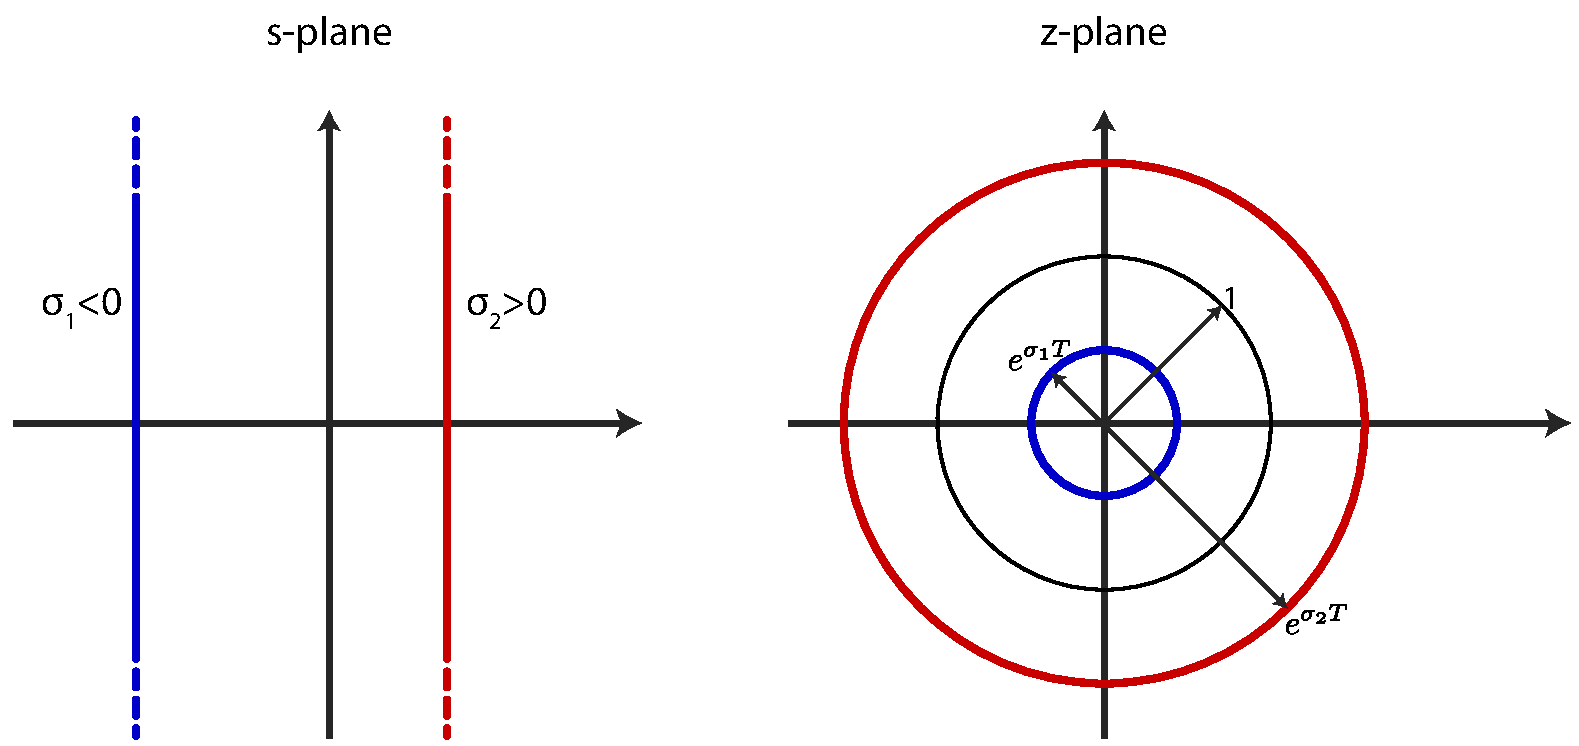
\includegraphics[width=\textwidth]{sigma}
    \end{center}
\end{minipage}
    \end{center}

\paragraph{Max convergence/settling time region:} For a stable 
CT LTI system convergence/settling time is defined by the 
real part of the pole. Thus on the s-plane we have the following 
condition
%
\begin{align*}
\mathrm{Re}(s) < \sigma_1 < 0 
\end{align*}
%
In the z-plane it is mapped to region enclosed by the 
circle with radius $r = e^{\sigma_1 T}$. This mapping is illustrated 
below.
%
    \begin{center}
\begin{minipage}[h]{0.85\linewidth}
    \begin{center}
      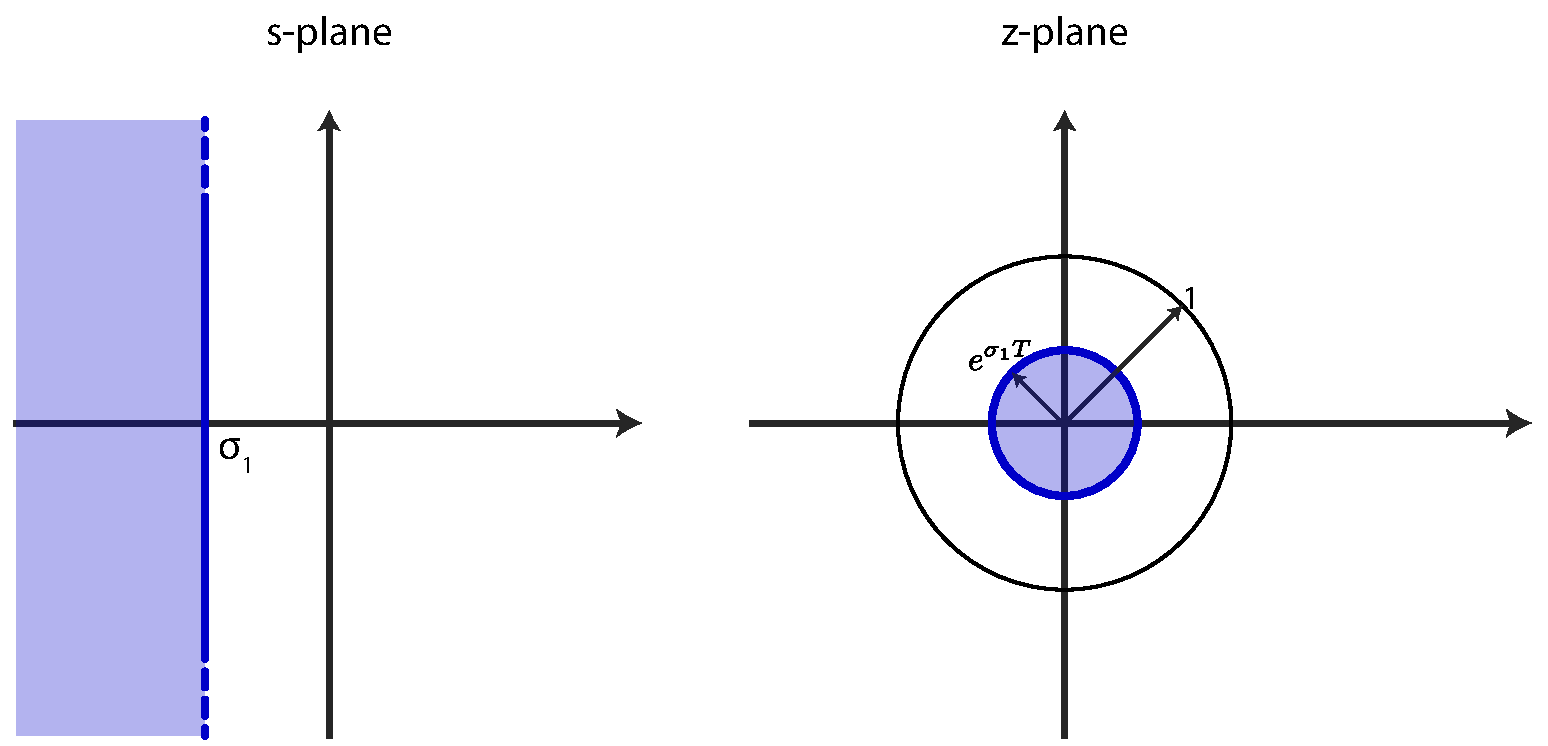
\includegraphics[width=\textwidth]{settling}
    \end{center}
\end{minipage}
    \end{center}
%
\paragraph{Constant frequency loci:} A constant frequency locus
$\omega = \omega_1$ in s-plane is mapped to a constant angle
line in z-plane, for which the angle is equal to $\omega_1 T$.
%
\begin{align*}
z &= e^{\sigma T} e^{\omega T j} =  e^{\sigma T} \angle \omega T\\
\angle \omega T &= \mathrm{Constant}
\end{align*}
%
Different constant frequency lines (all inside the primary strip) and
their mappings are illustrated in Figure below.
%
    \begin{center}
\begin{minipage}[h]{0.85\linewidth}
    \begin{center}
      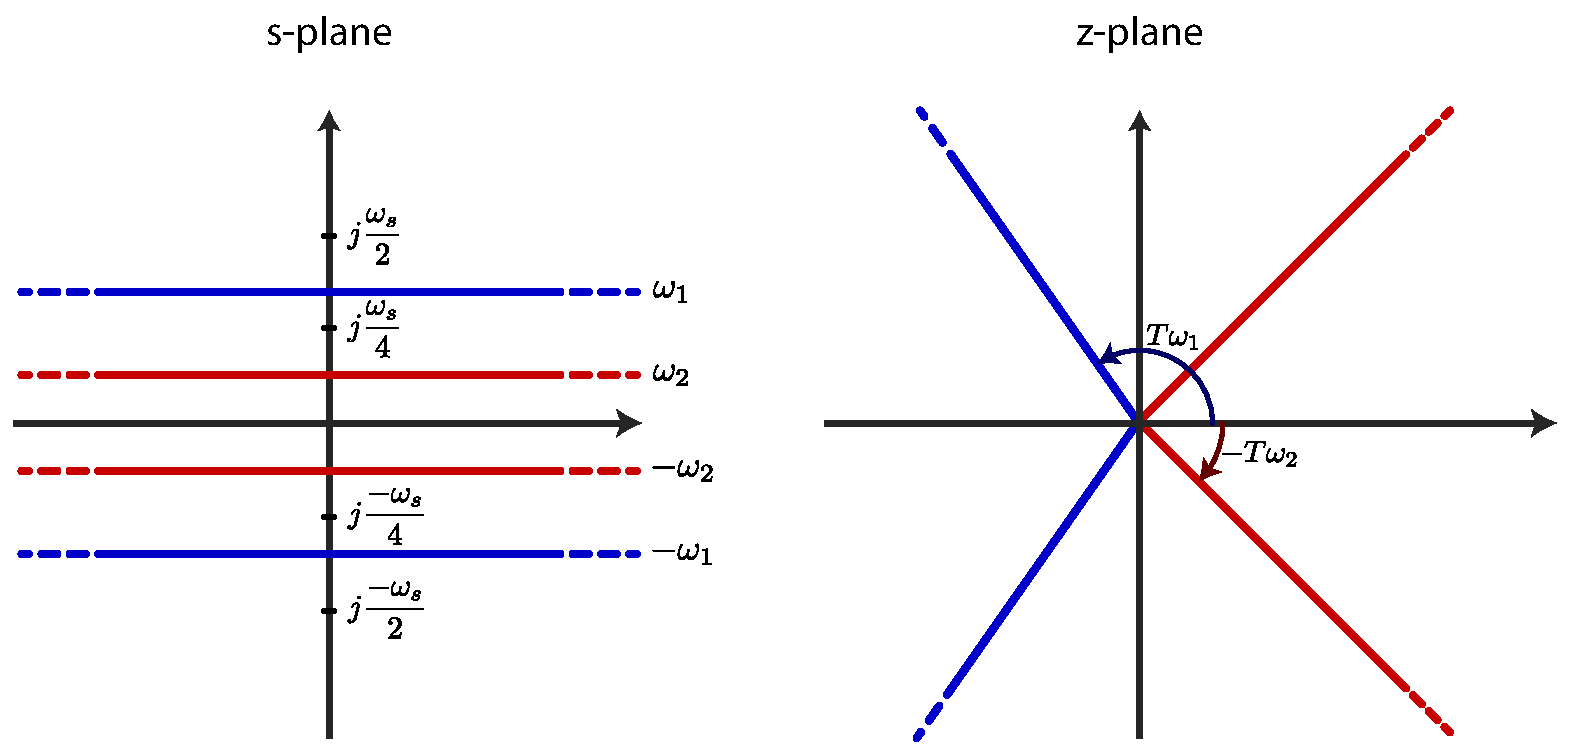
\includegraphics[width=\textwidth]{freq}
    \end{center}
\end{minipage}
    \end{center}
%
\textbf{Example:} Find the mapping of the area defined inside s-plane
illustrated in Figure below with $T=1$ .
%
    \begin{center}
\begin{minipage}[h]{0.5\linewidth}
    \begin{center}
      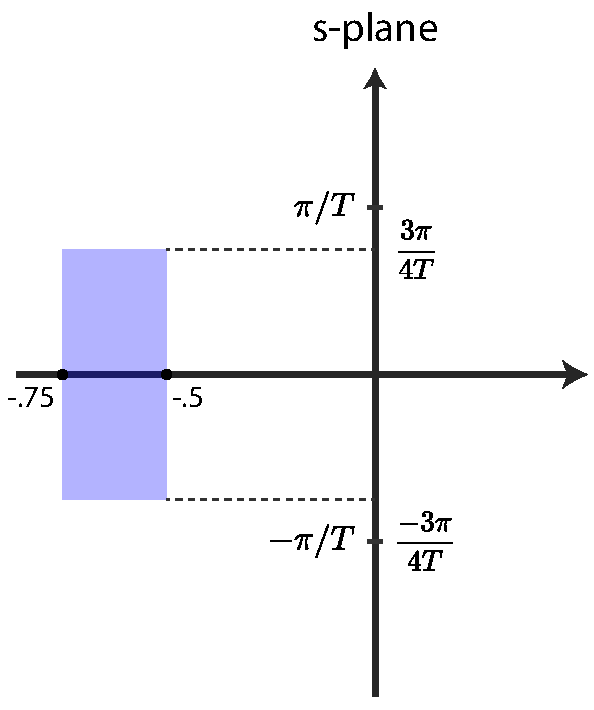
\includegraphics[width=\textwidth]{example}
    \end{center}
\end{minipage}
    \end{center}
%
\textbf{Solution:} The solution is illustrated in the Figure below
%
    \begin{center}
\begin{minipage}[h]{\linewidth}
    \begin{center}
      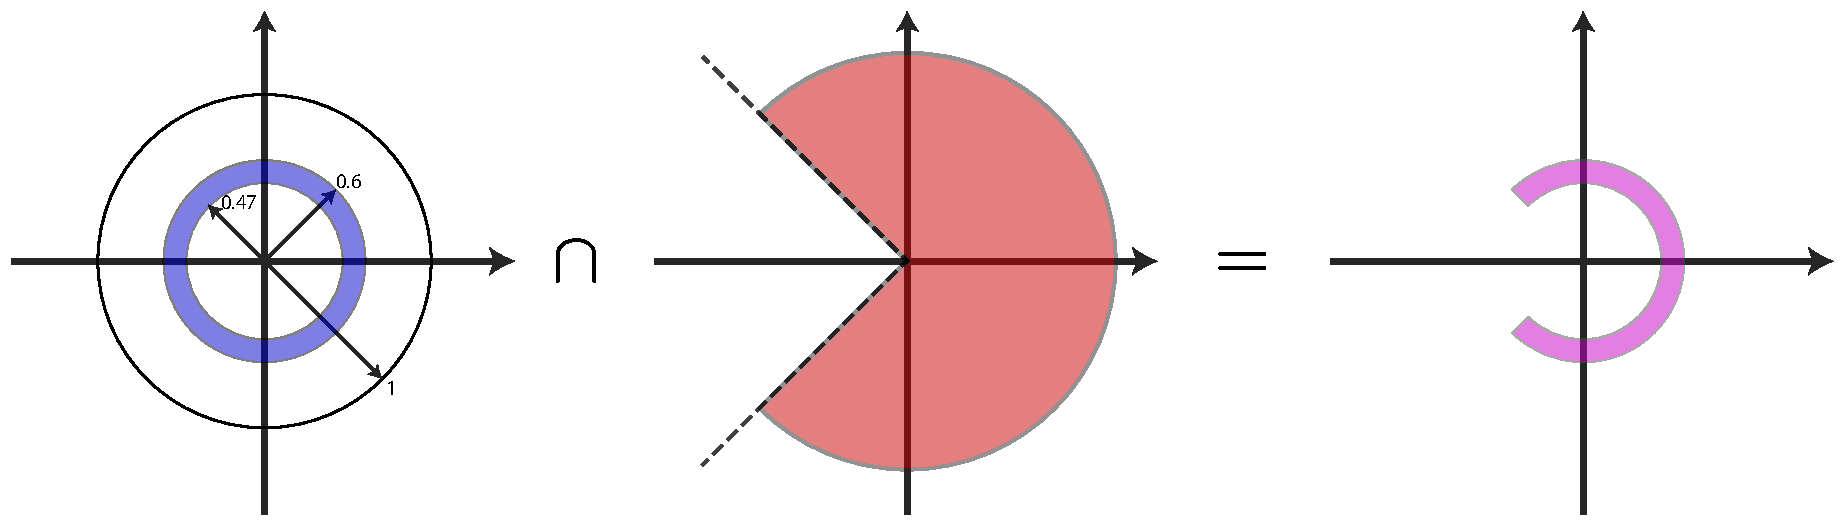
\includegraphics[width=\textwidth]{examplesol}
    \end{center}
\end{minipage}
    \end{center}
%
\paragraph{Constant damping loci:} A constant damping loci 
is a line in s-plane passing through the origin and the angle
between the line and the Real (or Imaginary) axis defines the damping 
ratio. In s-plane we have the following relations
%
\begin{align*}
s &= \sigma +\omega j = -\zeta \omega_n + \omega_n \sqrt{1 - \zeta^2} j \\
&= -\alpha \omega_d + j \omega_d
\\
\omega_d &=  \omega_n \sqrt{1 - \zeta^2}
\\
\alpha &= \frac{\zeta}{\sqrt{1 - \zeta^2}} = \mathrm{Constant} 
\end{align*}
%
The mapping of this line to the z-plane yields
%
\begin{align*}
z &= e^{-\alpha \omega_d T + j T \omega_d} = e^{-\alpha \omega_d T} 
  e^{j \omega_d T}\\
z &= e^{-2 \pi \alpha \frac{\omega_d}{\omega_s}} 
  e^{j 2 \pi \frac{\omega_d}{\omega_s}}
\\
|z| &= e^{-2 \pi \alpha \frac{\omega_d}{\omega_s}}
\\
\angle z &= 2 \pi \frac{\omega_d}{\omega_s}
\end{align*}
%
The curve in z-plane corresponds to a spiral shape as seen 
in Figure below.
%
    \begin{center}
\begin{minipage}[h]{\linewidth}
    \begin{center}
      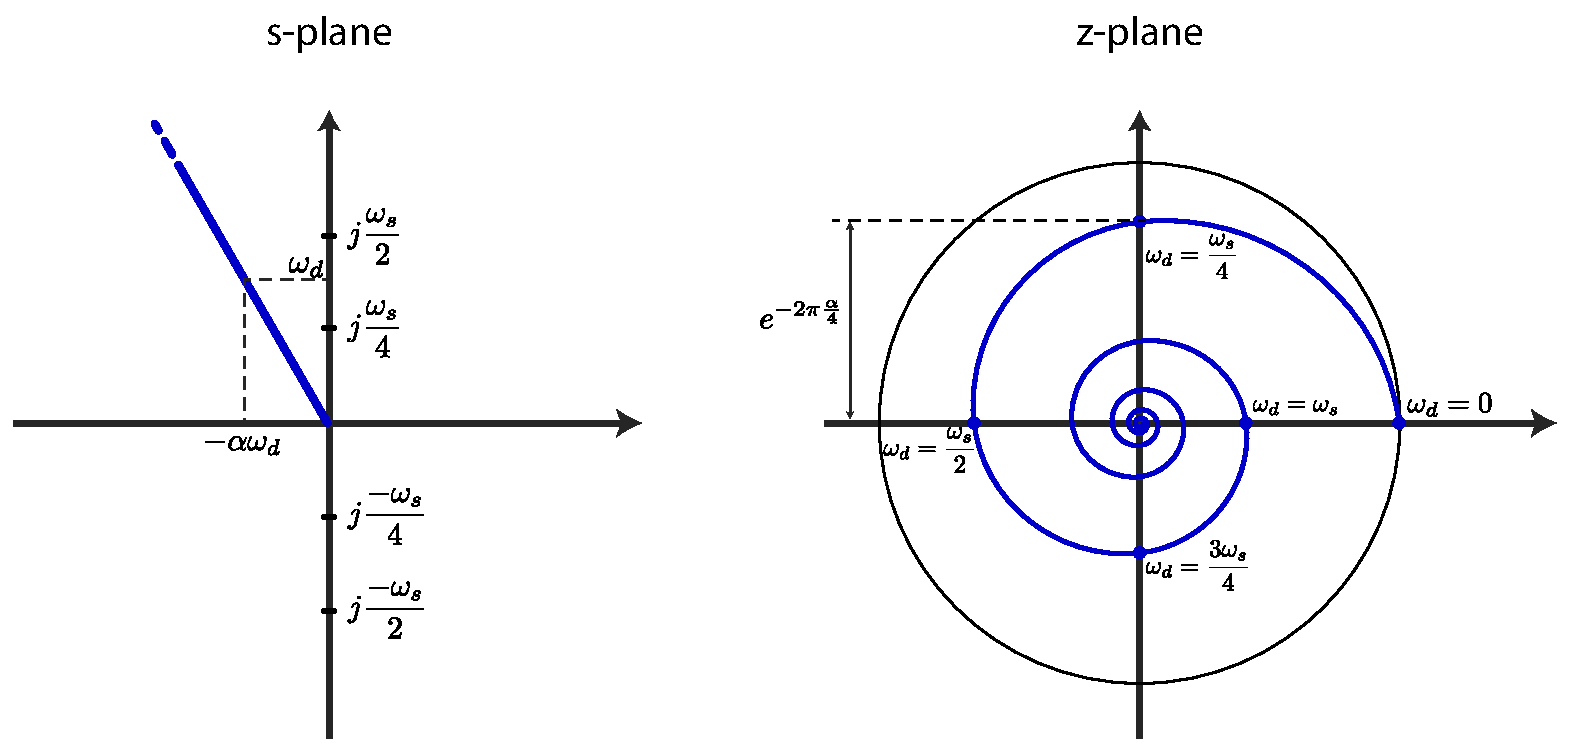
\includegraphics[width=\textwidth]{damping}
    \end{center}
\end{minipage}
    \end{center}
%
Note that for real systems we need to have also complex conjugates 
of both the line in s-plane and spiral in z-plane.


\textbf{Example:} Find the mapping of the area defined inside s-plane
illustrated in Figure below.
%
    \begin{center}
\begin{minipage}[h]{0.5\linewidth}
    \begin{center}
      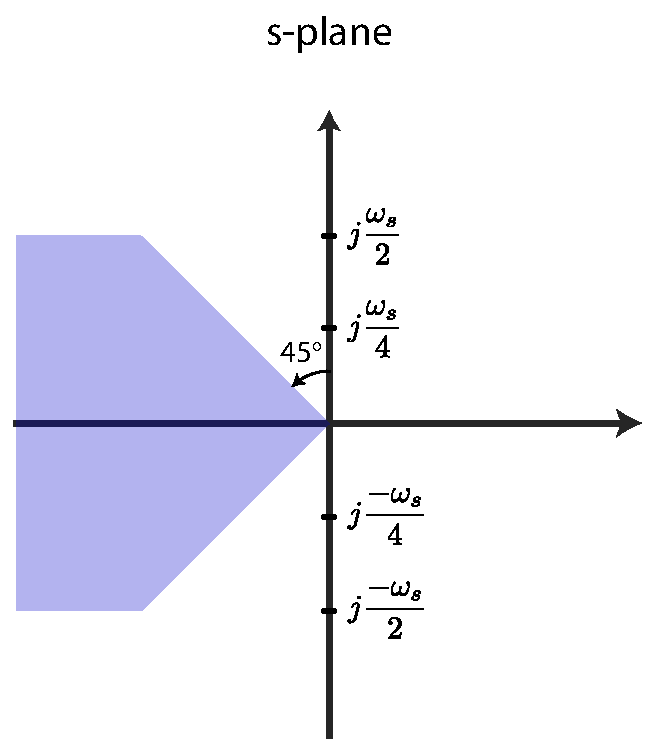
\includegraphics[width=\textwidth]{dampingexample}
    \end{center}
\end{minipage}
    \end{center}
%

\textbf{Solution:} The solution is illustrated in the Figure below
%
    \begin{center}
\begin{minipage}[h]{0.5\linewidth}
    \begin{center}
      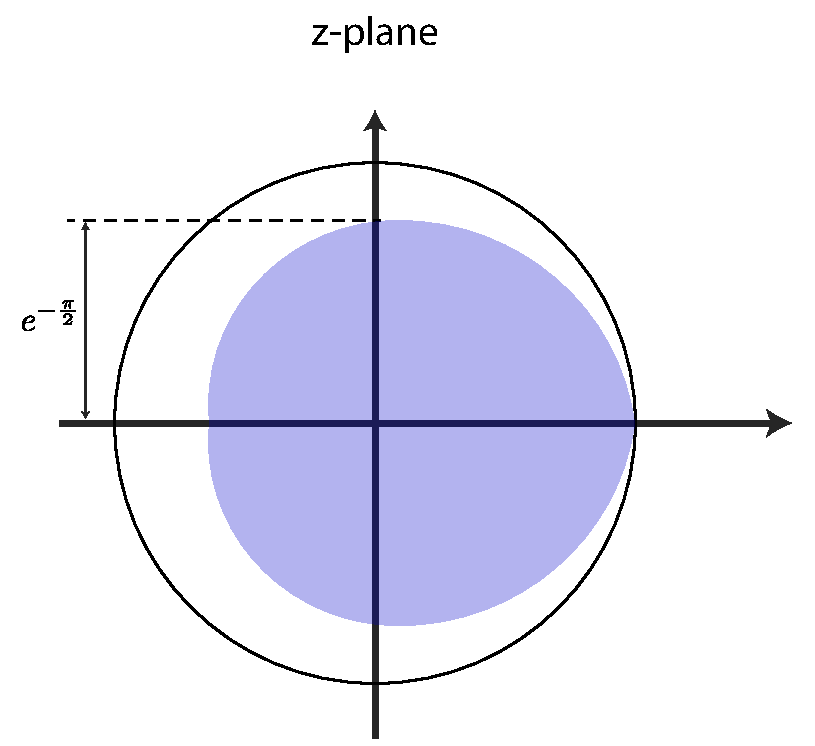
\includegraphics[width=\textwidth]{dampingexamplesol}
    \end{center}
\end{minipage}
    \end{center}

\section*{Bilinear Transformation}

A very common transformation used for design and analysis 
of discrete time control systems, digitized filters etc. is 
the bilinear transformation. It is a 1-1 mapping between 
complex z-plane and another complex plane $\bar{s}$ which 
is an ``imaginary'' s-domain plane. 

The bilinear transformation is defined by
%
\begin{align*}
 z &= \frac{1+\frac{T}{2} \bar{s}}{1-\frac{T}{2} \bar{s}} \\
 \bar{s} &= \frac{2}{T} \frac{z-1}{z+1}
\end{align*}
%
Let's analyze $|z| < 1$ 
%
\begin{align*}
|z| = \left| \frac{1+\frac{T}{2} \bar{s}}{1-\frac{T}{2} \bar{s}}
  \right| = \frac{| 1+\frac{T}{2} \bar{s} |}{| 1-\frac{T}{2} \bar{s}|
  }
\\
|z| < 1 \implies \left| 1+\frac{T}{2} \bar{s} \right| < \left|
  1-\frac{T}{2} \bar{s} \right|
\end{align*}
%
Let $\bar{s} = \bar{\sigma} + j \bar{\omega}$
%
\begin{align*}
\left| 1+\frac{T}{2} ( \bar{\sigma} + j \bar{\omega} ) \right| &<
  \left| 1-\frac{T}{2} ( \bar{\sigma} + j \bar{\omega} ) \right|
\\
\left( \frac{T}{2} \bar{\sigma} + 1 \right)^2 + \left( \frac{T}{2} \bar{\omega} \right)^2 
&<
\left( \frac{T}{2} \bar{\sigma} - 1 \right)^2 + \left( \frac{T}{2}
  \bar{\omega} \right)^2 
\\
\left( \frac{T}{2} \bar{\sigma} + 1 \right)^2 
&<
\left( \frac{T}{2} \bar{\sigma} - 1 \right)^2 \implies \bar{\sigma} < 0
\end{align*}
%
In other words we have the following relation 
%
\begin{align*}
  | z | < 1 \iff \mathrm{Re} \lbrace \bar{s}  \rbrace < 0
\end{align*}
%
which imples that tha area inside unit circle of z-plane (stable
region) is mapped to whole open left half plane of $\bar{s}$-plane.

Now let's consider the mapping of unit-cirlce on z-plane onto the 
$\bar{s}$-plane. 
%
\begin{align*}
  | z | = 1 \implies \left( \frac{T}{2} \bar{\sigma} + 1 \right)^2 
=
\left( \frac{T}{2} \bar{\sigma} - 1 \right)^2 \implies \bar{\sigma} = 0
\end{align*}
%
which imples that points on the unit circle are mapped to the
imaginary axis on the $\bar{s}$-plane. Now let's analyze this 
mapping further:
\begin{align*}
  | z | &= 1 \implies z = e^{j \omega_d} \ , \omega_d \in [-\pi , \pi]
\\
\bar{s} &= \frac{2}{T} \frac{e^{j \omega_d}-1}{e^{j \omega_d}+1} =   
\frac{2}{T} \frac{(e^{j \omega_d}-1)(e^{-j \omega_d}+1)}{(e^{j \omega_d}+1)(e^{-j \omega_d}+1)} =
j \frac{2}{T} \frac{ \sin \omega_d}{1 + \cos \omega_d}
= j \frac{2}{T} \frac{\sin (\omega_d/2) }{\cos (\omega_d/2)}
\\
\bar{\omega} &= \frac{2}{T} \tan (\omega_d/2)
\end{align*}
%
where $\bar{\omega}$ is the artificial frequency of the artificial CT system. 
If we analyze the frequency mapping we can easly see that
%
\begin{align*}
  \omega_d: \ 0 \to \pi \ &\implies \ \bar{\omega}: \ 0 \to \infty
\\
\omega_d: \ 0 \to -\pi \ &\implies \ \bar{\omega}: \ 0 \to -\infty
\end{align*}
%
Bilinear transformation and its basic mapping properties
are illustrated in the Figure below. 
%
    \begin{center}
\begin{minipage}[h]{0.8\linewidth}
    \begin{center}
      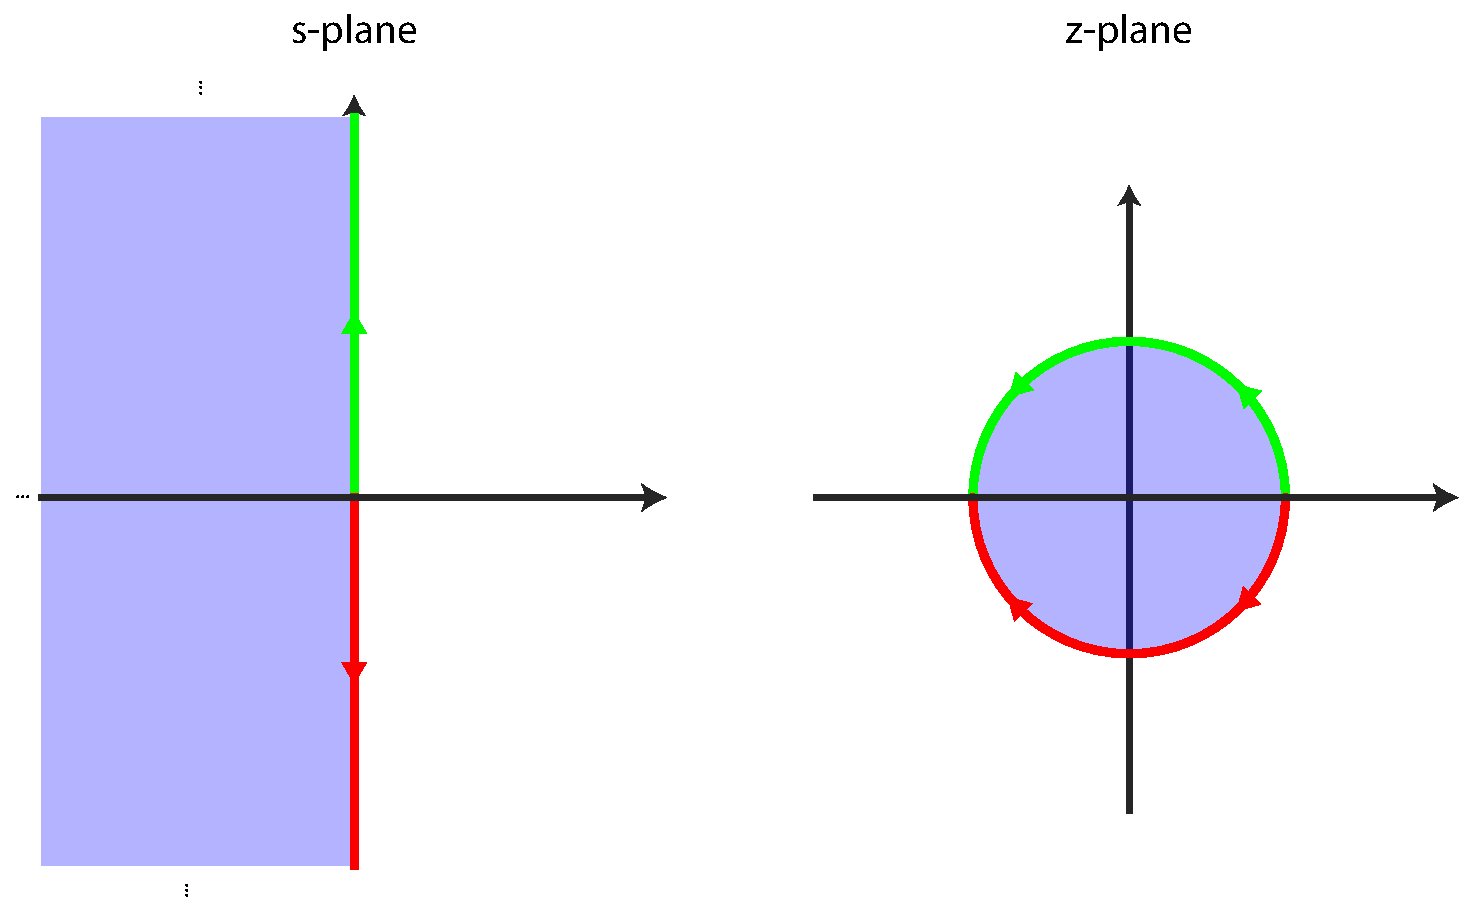
\includegraphics[width=\textwidth]{bilinear}
    \end{center}
\end{minipage}
    \end{center}
%
Blue transparent region corresponds to open left half
plane in $\bar{s}$-plane and area inside the unit 
circle in z-plane. Red and green lines/curves
illustrate the frequency paths in the respected
planes. 

Let's analyze the behavior of the frequency mapping around 
$\omega_d = 0$
%
\begin{align*}
\bar{\omega} &\approx \left[ \frac{d \bar{\omega}}{d \omega_d} 
\right]_{\omega_d} \omega_d = \omega_d / T 
\\ 
\bar{\omega} &\approx \omega_c
\end{align*}
%
where $\bar{\omega}$, $\omega_d$, and $\omega_c$ are 
the artificial CT-frequency, frequency in DT domain, and
actual frequency in CT domain respectively. The most important
relation is that at low frequencies $\bar{\omega} \approx \omega_c$.


In this linear region, the bilinear transformation behaves nicely
and we can roughly say that $G(s) \approx G(\bar{s})$. This means 
that bilinear transformation can be effectively used for design
of control systems, or measuring relative performance metrics
for the system of interest. However, as $\omega_d$ increases
there is a highly non-linear frequency wrapping (compression)
effect which can make both the design and analysis challenging
and sometimes even meaningless. 

The Figure below illustrates the relation between $\omega_d$
and $\omega$ as well as the linear approximation. 
%
    \begin{center}
\begin{minipage}[h]{0.4\linewidth}
    \begin{center}
      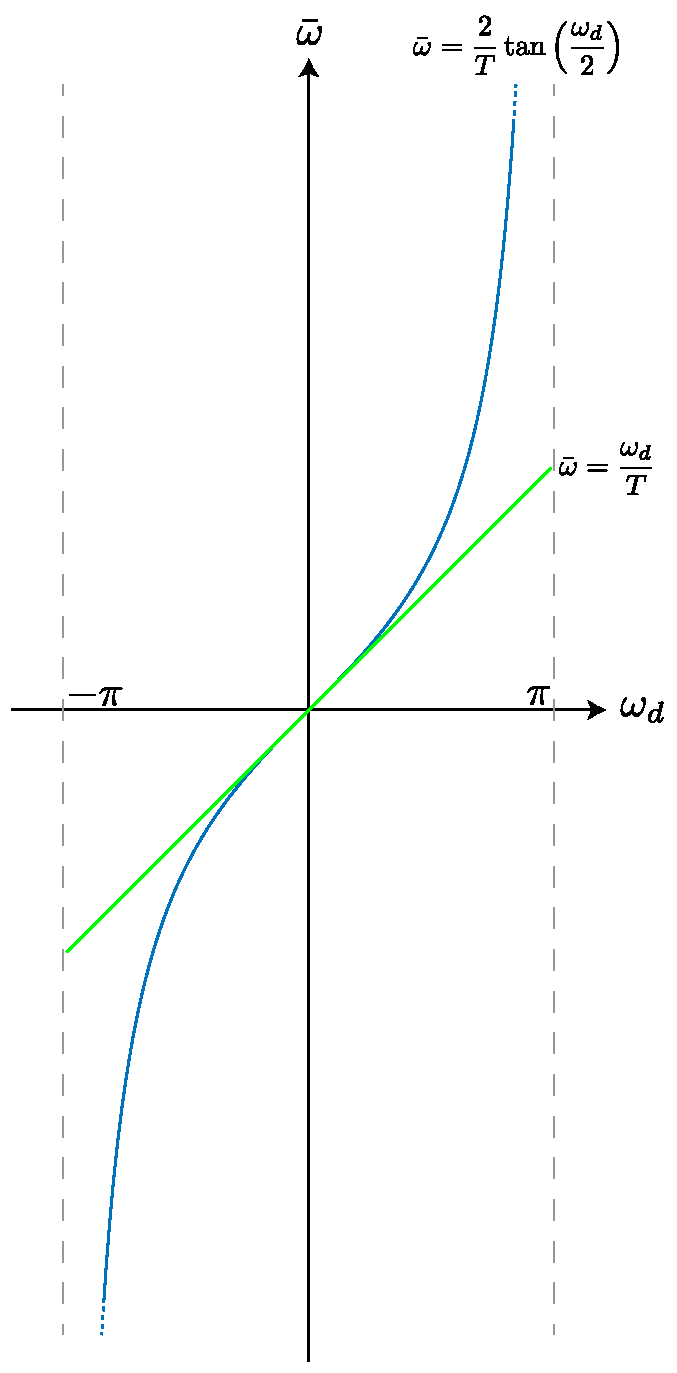
\includegraphics[width=\textwidth]{bifreq}
    \end{center}
\end{minipage}
    \end{center}
%

% **** This ENDS THE EXAMPLES. DON'T DELETE THE FOLLOWING LINE:
\end{document}